\documentclass[aspectratio=169]{beamer}
\usetheme{Singapore}
\usepackage[utf8]{inputenc}
\usepackage[T1]{fontenc}
\usepackage[french]{babel}
\usepackage{graphicx}

\definecolor{mainred}{RGB}{165,15,15}
\definecolor{darkred}{RGB}{100,5,5}
\setbeamercolor{structure}{fg=mainred}
\setbeamercolor{frametitle}{fg=darkred,bg=red!10}
\setbeamercolor{block title}{bg=mainred,fg=white}
\setbeamercolor{block body}{bg=red!5,fg=black}
\setbeamercolor{alerted text}{fg=darkred}

\graphicspath{{../}}   % les chemins figures_avalanche/xxx sont relatifs à presentation/

\begin{document}
% overlays 1..9
\begin{frame}[t]{Avalanche de sable — petite et grande}
\begin{columns}[T]
  \begin{column}{0.46\textwidth}
    \centering
    {\footnotesize\color{mainred}\textbf{Petite avalanche}}\\[0.2em]
      \only<1>{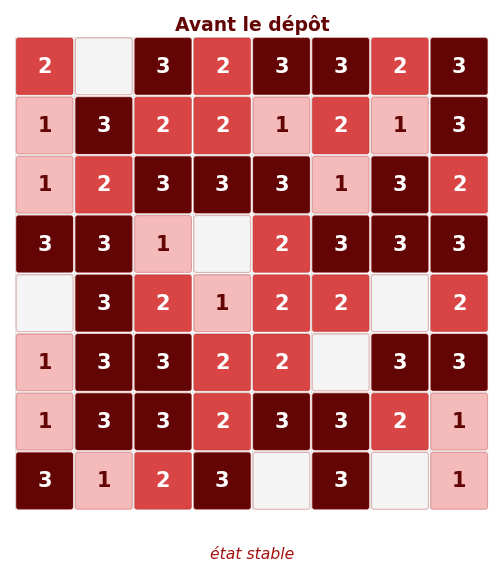
\includegraphics[width=\linewidth]{figures_avalanche/small_A0_avant.png}}
      \only<2>{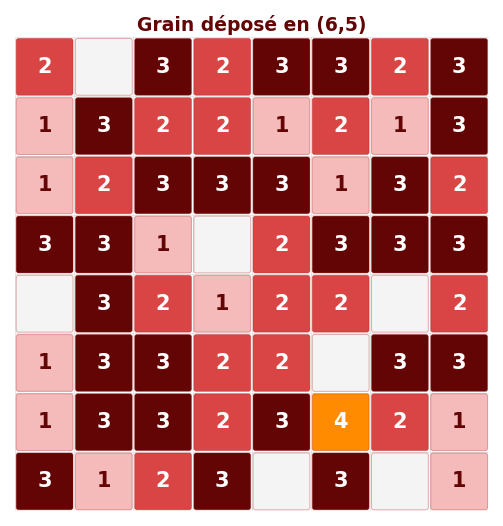
\includegraphics[width=\linewidth]{figures_avalanche/small_A1_depot.png}}
      \only<3>{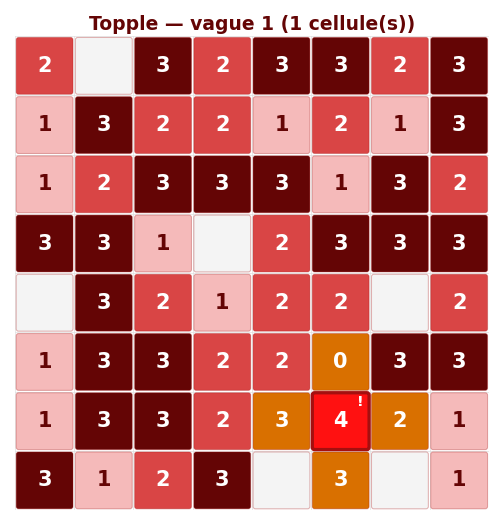
\includegraphics[width=\linewidth]{figures_avalanche/small_A2_topple.png}}
      \only<4>{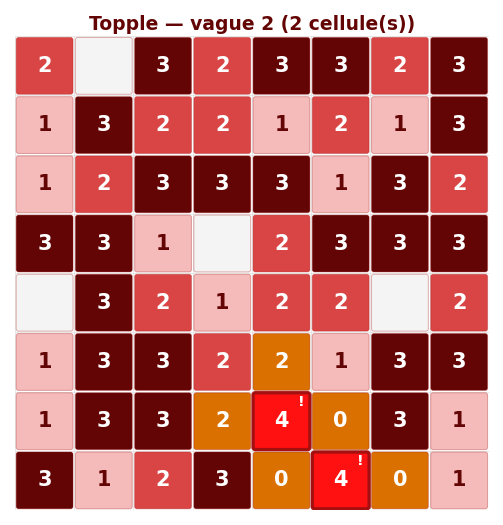
\includegraphics[width=\linewidth]{figures_avalanche/small_A3_topple.png}}
      \only<5->{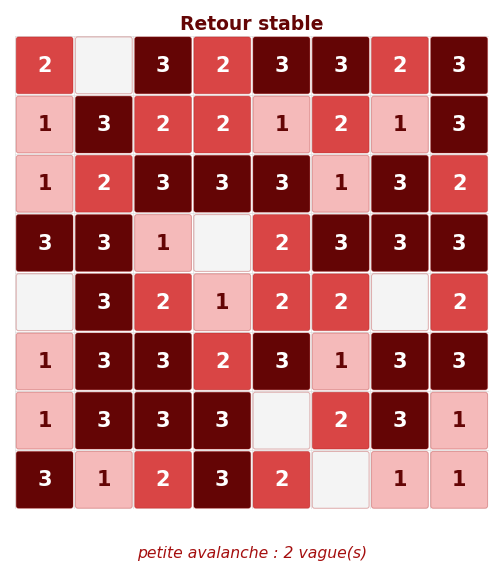
\includegraphics[width=\linewidth]{figures_avalanche/small_Afinal_stable.png}}
  \end{column}
  \begin{column}{0.46\textwidth}
    \centering
    {\footnotesize\color{mainred}\textbf{Grande avalanche}}\\[0.2em]
      \only<1>{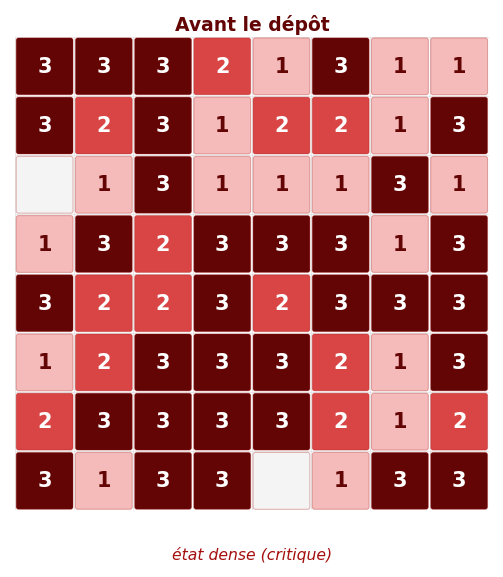
\includegraphics[width=\linewidth]{figures_avalanche/large_B0_avant.png}}
      \only<2>{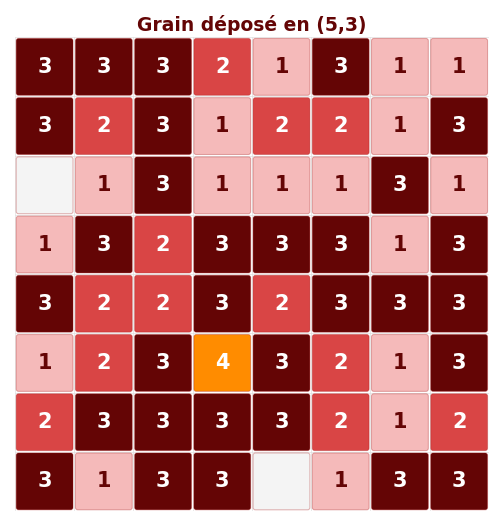
\includegraphics[width=\linewidth]{figures_avalanche/large_B1_depot.png}}
      \only<3>{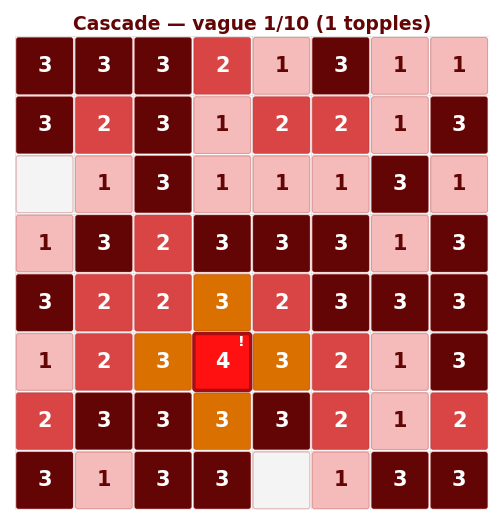
\includegraphics[width=\linewidth]{figures_avalanche/large_B2_wave.png}}
      \only<4>{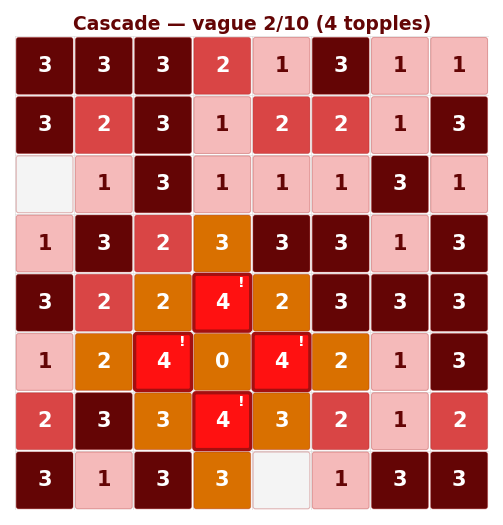
\includegraphics[width=\linewidth]{figures_avalanche/large_B3_wave.png}}
      \only<5>{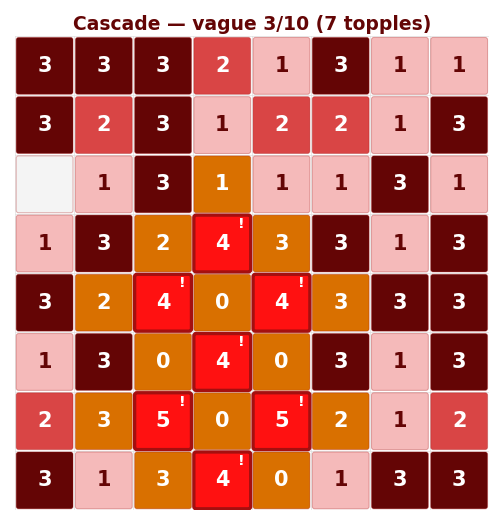
\includegraphics[width=\linewidth]{figures_avalanche/large_B4_wave.png}}
      \only<6>{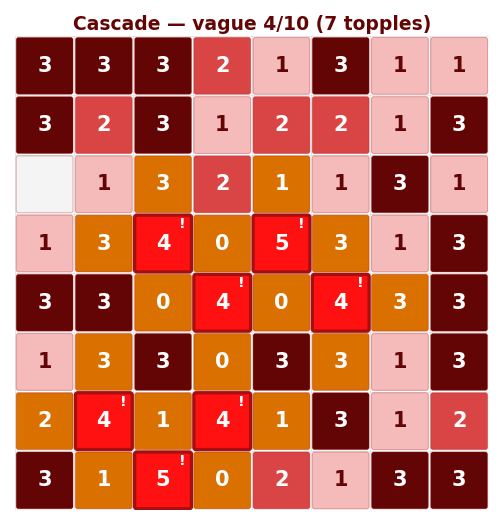
\includegraphics[width=\linewidth]{figures_avalanche/large_B5_wave.png}}
      \only<7>{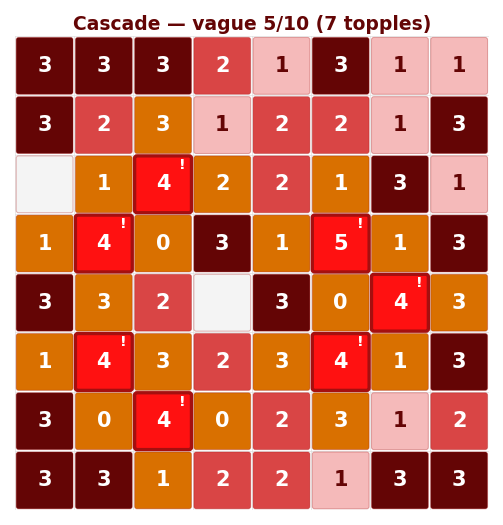
\includegraphics[width=\linewidth]{figures_avalanche/large_B6_wave.png}}
      \only<8>{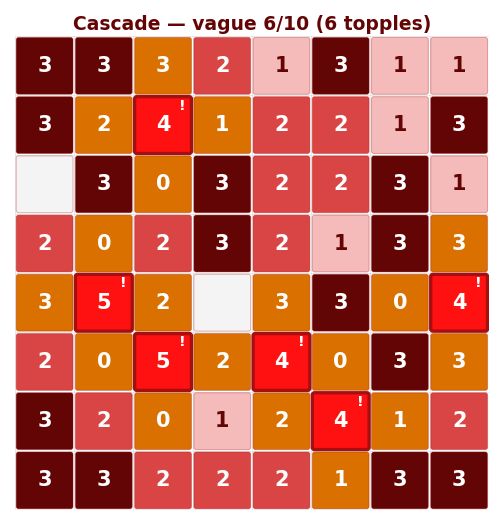
\includegraphics[width=\linewidth]{figures_avalanche/large_B7_wave.png}}
      \only<9->{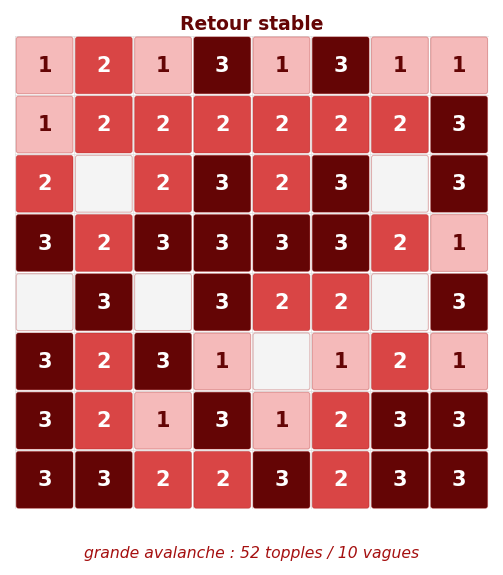
\includegraphics[width=\linewidth]{figures_avalanche/large_Bfinal_stable.png}}
  \end{column}
\end{columns}
\end{frame}

\begin{frame}{Distribution des avalanches}
\begin{center}
  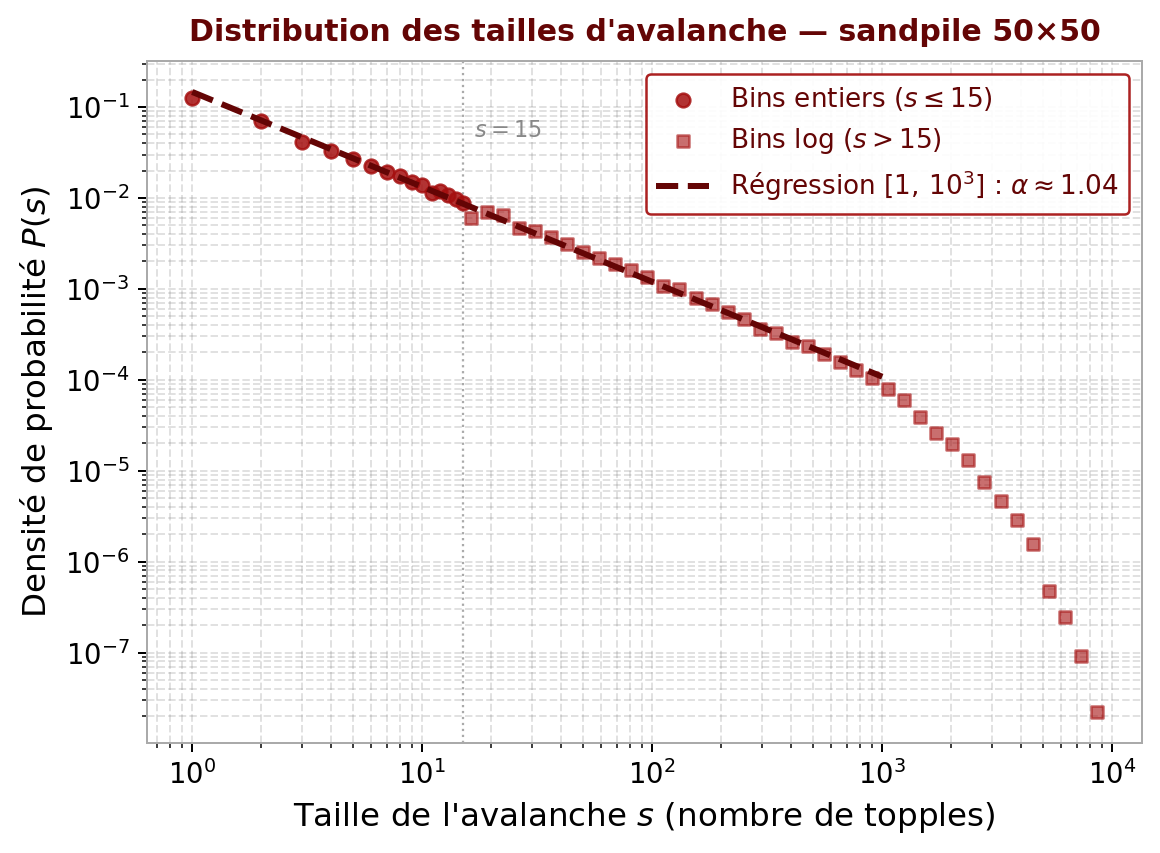
\includegraphics[width=0.80\textwidth]{figures_avalanche/powerlaw.png}
\end{center}
\begin{alertblock}{}
  \centering\small
  Distribution en \textbf{loi de puissance} $P(s)\sim s^{-\alpha}$,
  $\alpha \approx 1$ — \textbf{insensible} aux paramètres exogènes.
\end{alertblock}
\end{frame}

\end{document}
